\section{Galactic Anatomy}
\begin{center} 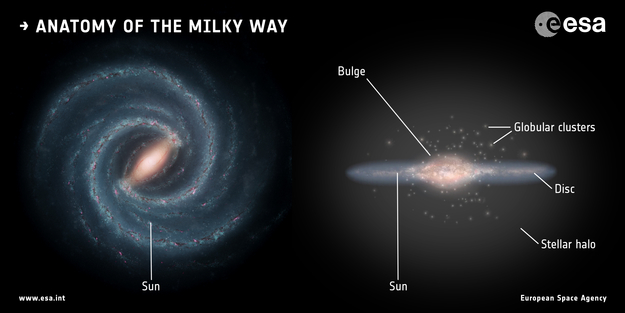
\includegraphics[scale=2]{galaxies/anatomy/pic} \end{center}
\begin{enumerate}
	\item the \textbf{bulge} is the huge, tightly packed group of stars found at the center of a spiral galaxy and as part of lenticular galaxies. there are generally considered to be 2 distinct kinds of bulges.
		\begin{enumerate}
			\item \textbf{classical bulges} have properties similar to elliptical galaxies.
				\begin{itemize}[noitemsep]
					\item comprised of older, redder, Population II stars.
					\item take on a spherical form due to composite stars having orbits which are random in comparison to the plane of the galaxy.
					\item no dust or gas $\rightarrow$ no star formation.
					\item the distribution of light is described by a Sersic profile.
					\item thought to be the results of smaller structures colliding, major mergers make gas clouds more likely to convert to stars.
					\item competing gravitational forces disrupt star orbit paths $\rightarrow$ random orbits.
					\item 80\% of galaxies lack a classical bulge, indicating they have never experienced a major merger.
					\item $\frac{2}{3}$ of galaxies in dense galaxy clusters possess a classical bulge, which demonstrates the disruptive effect of their crowding.
				\end{itemize}
			\item \textbf{disk-like bulges} have properties similar to the central regions of spiral galaxies. often referred to as pseudobulges or disky-bulges.
				\begin{itemize}[noitemsep]
					\item the stars orbit in an ordered fashion in the same plane as the stars in the outer disk.
					\item these bulges have varied structures similar in appearance to spiral galaxies, but 2-100 times smaller.
					\item the rate at which new stars are formed in these bulges is similar to the rate at which stars form in disc galaxies. bulges may contain nuclear rings that are forming stars at much higher rate (per area) than is typically found in outer disks.
					\item theories regarding their formation are uncertain.
						\begin{itemize}[noitemsep]
							\item may be the result of gas-rich mergers which happened more recently (last 5 billion years) than classical bulges, but it is difficult for disks to survive mergers, making this doubtful.
							\item disk galaxies can rearrange their stars and gas in response to instabilities (secular evolution). this process is believed to send gas and dust to the center of a galaxy, increasing the density and creating a bulge.
						\end{itemize}
				\end{itemize}
			\item most bulges and pseudo-bulges are thought to host a central relativistic compact mass, which is traditionally assumed to be a supermassive black hole.
				\begin{itemize}[noitemsep]
					\item  masses of the black holes correlate tightly with bulge properties.
					\item M-sigma relation relates black hole mass to the velocity dispersion of bulge stars
					\item total stellar mass
					\item luminosity
					\item central concentration of stars
					\item  richness of the globular cluster system orbiting in the galaxy's far outskirts
					\item angle of spiral arms
				\end{itemize}
		\end{enumerate}
	\item the \textbf{disc} is a component of disc galaxies (spiral and lenticular). discs consist of 2 components. they tend to be flat, since the orbits of their components tend to be focused in 1 plane, with little vertical motion.
		\begin{enumerate}
			\item the \textbf{stellar component} is composed of most of the galaxy's stars.
				\begin{itemize}[noitemsep]
					\item tends to exhibit little random motions; stars undergo mostly circular orbits around the center.
					\item this leads to the formation of spiral arms in spiral galaxies.
				\end{itemize}
			\item the \textbf{gaseous component} is composed mostly of cool gas and dust.
				\begin{itemize}[noitemsep]
					\item majority of the gaseous component is cool atomic hydrogen (HI) and warm atomic hydrogen (HII). hydrogen is distributed fairly uniformly throughout the disc.
					\item gas serves as fuel for the formation of new stars in the disc.
					\item 21-cm emission by HI shows that the gaseous component can flare at the outer region of the galaxy.
					\item clumps or clouds of gas follow approximately circular orbits about the galactic center.
					\item circular velocity of the gas in the disc is strongly correlated with the luminosity of the galaxy (see Tully-Fisher Relation).
				\end{itemize}
		\end{enumerate}
	\item the \textbf{halo} is an extended, roughly spherical component of a galaxy which extends beyond the main, visible component. The distinction between the halo and the main body of the galaxy is clearest in spiral galaxies, where the spherical shape of the halo contrasts with the flat disc. In an elliptic al galaxy, there is no sharp transition between the other components of the galaxy and the halo.
		\begin{enumerate}
			\item the \textbf{stellar halo} is the component of the halo containing the stars.
				\begin{itemize}[noitemsep]
					\item typically contains oldest, most metal stars.
					\item since they are so faint, studying stellar halos requires very long exposure times.
					\item data from many galaxies must be combined to derive the average properties of a stellar halo. it is only possible to measure individual stars in the Andromeda and Milky Way galaxies.
					\item the furthest stellar halos detected are at a redshift distance of 1.
					\item it is thought that stellar halos consist both of natively created stars and stars obtained from satellite galaxies which merged. this results in streams of stars which are coherent in space or velocity due to being from the same galaxy, as well as variations in properties like metallicity across the halo as a whole.
					\item it is thought that the Milky Way's stellar halo contains 0.1-1\% of its stellar mass.
				\end{itemize}
			\item the \textbf{galactic corona} is the hot, ionized, gaseous component of the galactic halo.
				\begin{itemize}[noitemsep]
					\item coronal gas may be sustained by the \textbf{galactic fountain} --- superbubbles of ionized gas from supernova remnants expands vertically through galactic chimneys into the halo.
					\item as the gas cools, it is eventually pulled back into the disc.
				\end{itemize}
			\item the \textbf{dark matter halo} is a hypothetical part of a galaxy which envelops the galactic disc and extends beyond the edge of the visible galaxy.
				\begin{itemize}[noitemsep]
					\item the presence of dark matter is inferred from its gravitational effect.
						\begin{itemize}[noitemsep]
							\item w/o large amounts of mass throughout the halo, the rotational velocity of the galaxy would decrease the farther it is from the galactic center
							\item however, the rotation curve of most spiral galaxies flattens out.
							\item the absence of visible matter to account for this implies that unobserved, i.e. dark, matter causes it (or that general relativity is incomplete).
						\end{itemize}
					\item dark matter halos are believed to have played a large role in the formation of the early universe.
						\begin{itemize}[noitemsep]
							\item during initial formation, the temperature of the baryonic matter should have still been too high for it to form gravitationally-bound objects alone $\rightarrow$ dark matter structures must have added additional gravitational force b/c dark matter is cold compared to baryonic matter.
							\item hypothesis for CDM structure formation begins with density perturbations in the Universe that grow linearly until they reach a critical density, after which they would stop expanding and collapse to form gravitationally bound dark matter halos. These halos would continue to grow in mass (and size), either through accretion of material from their immediate neighborhood, or by merging with other halos.
						\end{itemize}
				\end{itemize}
		\end{enumerate}
\end{enumerate}